\documentclass[ignorenonframetext,]{beamer}
\setbeamertemplate{caption}[numbered]
\setbeamertemplate{caption label separator}{: }
\setbeamercolor{caption name}{fg=normal text.fg}
\beamertemplatenavigationsymbolsempty
\usepackage{lmodern}
\usepackage{amssymb,amsmath}
\usepackage{ifxetex,ifluatex}
\usepackage{fixltx2e} % provides \textsubscript
\ifnum 0\ifxetex 1\fi\ifluatex 1\fi=0 % if pdftex
  \usepackage[T1]{fontenc}
  \usepackage[utf8]{inputenc}
\else % if luatex or xelatex
  \ifxetex
    \usepackage{mathspec}
  \else
    \usepackage{fontspec}
  \fi
  \defaultfontfeatures{Ligatures=TeX,Scale=MatchLowercase}
\fi
% use upquote if available, for straight quotes in verbatim environments
\IfFileExists{upquote.sty}{\usepackage{upquote}}{}
% use microtype if available
\IfFileExists{microtype.sty}{%
\usepackage{microtype}
\UseMicrotypeSet[protrusion]{basicmath} % disable protrusion for tt fonts
}{}
\newif\ifbibliography
\hypersetup{
            pdftitle={clase 5 de Mayo},
            pdfauthor={Mariano Dominguez},
            pdfborder={0 0 0},
            breaklinks=true}
\urlstyle{same}  % don't use monospace font for urls
\usepackage{color}
\usepackage{fancyvrb}
\newcommand{\VerbBar}{|}
\newcommand{\VERB}{\Verb[commandchars=\\\{\}]}
\DefineVerbatimEnvironment{Highlighting}{Verbatim}{commandchars=\\\{\}}
% Add ',fontsize=\small' for more characters per line
\usepackage{framed}
\definecolor{shadecolor}{RGB}{248,248,248}
\newenvironment{Shaded}{\begin{snugshade}}{\end{snugshade}}
\newcommand{\KeywordTok}[1]{\textcolor[rgb]{0.13,0.29,0.53}{\textbf{#1}}}
\newcommand{\DataTypeTok}[1]{\textcolor[rgb]{0.13,0.29,0.53}{#1}}
\newcommand{\DecValTok}[1]{\textcolor[rgb]{0.00,0.00,0.81}{#1}}
\newcommand{\BaseNTok}[1]{\textcolor[rgb]{0.00,0.00,0.81}{#1}}
\newcommand{\FloatTok}[1]{\textcolor[rgb]{0.00,0.00,0.81}{#1}}
\newcommand{\ConstantTok}[1]{\textcolor[rgb]{0.00,0.00,0.00}{#1}}
\newcommand{\CharTok}[1]{\textcolor[rgb]{0.31,0.60,0.02}{#1}}
\newcommand{\SpecialCharTok}[1]{\textcolor[rgb]{0.00,0.00,0.00}{#1}}
\newcommand{\StringTok}[1]{\textcolor[rgb]{0.31,0.60,0.02}{#1}}
\newcommand{\VerbatimStringTok}[1]{\textcolor[rgb]{0.31,0.60,0.02}{#1}}
\newcommand{\SpecialStringTok}[1]{\textcolor[rgb]{0.31,0.60,0.02}{#1}}
\newcommand{\ImportTok}[1]{#1}
\newcommand{\CommentTok}[1]{\textcolor[rgb]{0.56,0.35,0.01}{\textit{#1}}}
\newcommand{\DocumentationTok}[1]{\textcolor[rgb]{0.56,0.35,0.01}{\textbf{\textit{#1}}}}
\newcommand{\AnnotationTok}[1]{\textcolor[rgb]{0.56,0.35,0.01}{\textbf{\textit{#1}}}}
\newcommand{\CommentVarTok}[1]{\textcolor[rgb]{0.56,0.35,0.01}{\textbf{\textit{#1}}}}
\newcommand{\OtherTok}[1]{\textcolor[rgb]{0.56,0.35,0.01}{#1}}
\newcommand{\FunctionTok}[1]{\textcolor[rgb]{0.00,0.00,0.00}{#1}}
\newcommand{\VariableTok}[1]{\textcolor[rgb]{0.00,0.00,0.00}{#1}}
\newcommand{\ControlFlowTok}[1]{\textcolor[rgb]{0.13,0.29,0.53}{\textbf{#1}}}
\newcommand{\OperatorTok}[1]{\textcolor[rgb]{0.81,0.36,0.00}{\textbf{#1}}}
\newcommand{\BuiltInTok}[1]{#1}
\newcommand{\ExtensionTok}[1]{#1}
\newcommand{\PreprocessorTok}[1]{\textcolor[rgb]{0.56,0.35,0.01}{\textit{#1}}}
\newcommand{\AttributeTok}[1]{\textcolor[rgb]{0.77,0.63,0.00}{#1}}
\newcommand{\RegionMarkerTok}[1]{#1}
\newcommand{\InformationTok}[1]{\textcolor[rgb]{0.56,0.35,0.01}{\textbf{\textit{#1}}}}
\newcommand{\WarningTok}[1]{\textcolor[rgb]{0.56,0.35,0.01}{\textbf{\textit{#1}}}}
\newcommand{\AlertTok}[1]{\textcolor[rgb]{0.94,0.16,0.16}{#1}}
\newcommand{\ErrorTok}[1]{\textcolor[rgb]{0.64,0.00,0.00}{\textbf{#1}}}
\newcommand{\NormalTok}[1]{#1}
\usepackage{graphicx,grffile}
\makeatletter
\def\maxwidth{\ifdim\Gin@nat@width>\linewidth\linewidth\else\Gin@nat@width\fi}
\def\maxheight{\ifdim\Gin@nat@height>\textheight0.8\textheight\else\Gin@nat@height\fi}
\makeatother
% Scale images if necessary, so that they will not overflow the page
% margins by default, and it is still possible to overwrite the defaults
% using explicit options in \includegraphics[width, height, ...]{}
\setkeys{Gin}{width=\maxwidth,height=\maxheight,keepaspectratio}

% Prevent slide breaks in the middle of a paragraph:
\widowpenalties 1 10000
\raggedbottom

\AtBeginPart{
  \let\insertpartnumber\relax
  \let\partname\relax
  \frame{\partpage}
}
\AtBeginSection{
  \ifbibliography
  \else
    \let\insertsectionnumber\relax
    \let\sectionname\relax
    \frame{\sectionpage}
  \fi
}
\AtBeginSubsection{
  \let\insertsubsectionnumber\relax
  \let\subsectionname\relax
  \frame{\subsectionpage}
}

\setlength{\parindent}{0pt}
\setlength{\parskip}{6pt plus 2pt minus 1pt}
\setlength{\emergencystretch}{3em}  % prevent overfull lines
\providecommand{\tightlist}{%
  \setlength{\itemsep}{0pt}\setlength{\parskip}{0pt}}
\setcounter{secnumdepth}{0}

\title{clase 5 de Mayo}
\author{Mariano Dominguez}
\date{April 29, 2018}

\begin{document}
\frame{\titlepage}

\begin{frame}{Análisis exploratorio y curación de datos}

\begin{itemize}
\tightlist
\item
  Mariano Dominguez @ IATE-OAC-UNC \& CONICET
\item
  Edgardo Hames @ Bitlogic
\item
  Gabriel Miretti @ Bitlogic
\end{itemize}

\begin{figure}
\centering

\includegraphics{./logos-diplomatura-3.png}
\caption{Diplodatos @ FaMAF}
\end{figure}

\end{frame}

\begin{frame}

\begin{block}{Un breve vistazo de Aprendizaje supervisado}

\begin{itemize}
\item
  Tenemos un conjunto de variables medidas que las llamaremos
  \textbf{inputs}. Estas tienen alguna influencia en una o mas variables
  que llamaremos \textbf{outputs}. La \textbf{meta} es utilizar los
  inputs \textbf{para predecir} los valores de los outputs.
\item
  En la literatura estadistica los inputs son frecuentemente llamados
  como \textbf{predictores}, un termino que puede usarse
  equivalentemente a inputs, y mas clasicamente seran las
  \textbf{variables independientes}.
\item
  En la literatura de reconocimiento de patrones se prefiere el termino
  \textbf{features} . Los outputs son llamados tambien las
  \textbf{respuestas}, o clasicamente las \textbf{variables
  dependientes}.
\end{itemize}

\end{block}

\end{frame}

\begin{frame}

\begin{block}{Modelos Lineales y Cuadrados minimos}

Los modelos lineales son una de las herramientas estadisticas mas
importantes. Dado un vector de inputs
\(X^{T}=(X_{1}, X_{2}, ..., X_{p})\), se puede predecir el output \(Y\)
via el siguiente modelo:
\(\hat{Y} = \hat{ \beta_{0} } + \sum_{j=1}^{p} X_{j} \hat{ \beta_{j}}\)

\(\hat{\beta_{0}}\) es la ordenada al origen, tambien conocida como el
\textbf{bias} en aprendizaje automatico (machine learning). A menudo es
conveniente incluir la variable constante 1 en \(X\), y de manera
similar \(\hat{\beta_{0}}\) en el vector de coeficientes
\(\hat{\beta}\), y entonces escribir el modelo lineal en forma de un
producto interno vectorial: \(\hat{Y}=X^{T}\hat{\beta}\).

Especificar modelos estadisticos como regresion es muy simple en R.
Simplemente escribiendo ``y \textasciitilde{} model'', donde ``y'' sera
la variable de respuesta y model seran todos los predictores a ser
incluidos en el modelo. Para la regresion lineal utilizaremos la funcion
lm.

\end{block}

\end{frame}

\begin{frame}[fragile]

\begin{block}{Una simple Regresion Lineal 1:}

Utilizaremos un conjunto de datos de 92 estrellas del grupo de las
Hyades las cuales filtraremos por coordenadas y errores de medicion en
la paralaje.

\begin{Shaded}
\begin{Highlighting}[]
\NormalTok{loc <-}\StringTok{ "http://astrostatistics.psu.edu/datasets/"}
\NormalTok{hip <-}\StringTok{ }\KeywordTok{read.table}\NormalTok{(}\KeywordTok{paste}\NormalTok{(loc,}\StringTok{"HIP_star.dat"}\NormalTok{,}\DataTypeTok{sep=}\StringTok{""}\NormalTok{),}
\DataTypeTok{header=}\NormalTok{T,}\DataTypeTok{fill=}\NormalTok{T)}
\KeywordTok{attach}\NormalTok{(hip)}
\NormalTok{filter1 <-}\StringTok{ }\NormalTok{(RA}\OperatorTok{>}\DecValTok{50} \OperatorTok{&}\StringTok{ }\NormalTok{RA}\OperatorTok{<}\DecValTok{100} \OperatorTok{&}\StringTok{ }\NormalTok{DE}\OperatorTok{>}\DecValTok{0} \OperatorTok{&}\StringTok{ }\NormalTok{DE}\OperatorTok{<}\DecValTok{25}\NormalTok{)}
\NormalTok{filter2 <-}\StringTok{ }\NormalTok{(pmRA}\OperatorTok{>}\DecValTok{90} \OperatorTok{&}\StringTok{ }\NormalTok{pmRA}\OperatorTok{<}\DecValTok{130} \OperatorTok{&}\StringTok{ }\NormalTok{pmDE}\OperatorTok{>-}\DecValTok{60} \OperatorTok{&}\StringTok{ }\NormalTok{pmDE}\OperatorTok{<}\StringTok{ }\OperatorTok{-}\DecValTok{10}\NormalTok{)}
\NormalTok{filter <-}\StringTok{ }\NormalTok{filter1 }\OperatorTok{&}\StringTok{ }\NormalTok{filter2 }\OperatorTok{&}\StringTok{ }\NormalTok{(e_Plx}\OperatorTok{<}\DecValTok{5}\NormalTok{)}
\KeywordTok{sum}\NormalTok{(filter)}
\end{Highlighting}
\end{Shaded}

\begin{verbatim}
## [1] 92
\end{verbatim}

\end{block}

\end{frame}

\begin{frame}[fragile]

\begin{block}{Una simple Regresion Lineal 2:}

Un breve ejemplo de una regresion linear entre \(B-V\) y \(\log(L)\).

\begin{Shaded}
\begin{Highlighting}[]
\NormalTok{mainseqhyades <-}\StringTok{ }\NormalTok{filter }\OperatorTok{&}\StringTok{ }\NormalTok{(Vmag}\OperatorTok{>}\DecValTok{4} \OperatorTok{|}\StringTok{ }\NormalTok{B.V}\OperatorTok{<}\FloatTok{0.2}\NormalTok{)}
\NormalTok{logL <-}\StringTok{ }\NormalTok{(}\DecValTok{15}\OperatorTok{-}\NormalTok{Vmag}\OperatorTok{-}\DecValTok{5} \OperatorTok{*}\StringTok{ }\KeywordTok{log10}\NormalTok{(Plx)) }\OperatorTok{/}\StringTok{ }\FloatTok{2.5}
\NormalTok{x <-}\StringTok{ }\NormalTok{logL[mainseqhyades]}
\NormalTok{y <-}\StringTok{ }\NormalTok{B.V[mainseqhyades]}
\NormalTok{regline <-}\StringTok{ }\KeywordTok{lm}\NormalTok{(y}\OperatorTok{~}\NormalTok{x)}
\KeywordTok{summary}\NormalTok{(regline)}
\end{Highlighting}
\end{Shaded}

\begin{verbatim}
## 
## Call:
## lm(formula = y ~ x)
## 
## Residuals:
##      Min       1Q   Median       3Q      Max 
## -0.08578 -0.04846 -0.01741  0.04004  0.22711 
## 
## Coefficients:
##              Estimate Std. Error t value Pr(>|t|)    
## (Intercept)  0.746857   0.007712   96.85   <2e-16 ***
## x           -0.405698   0.009148  -44.35   <2e-16 ***
## ---
## Signif. codes:  0 '***' 0.001 '**' 0.01 '*' 0.05 '.' 0.1 ' ' 1
## 
## Residual standard error: 0.06487 on 86 degrees of freedom
## Multiple R-squared:  0.9581, Adjusted R-squared:  0.9576 
## F-statistic:  1967 on 1 and 86 DF,  p-value: < 2.2e-16
\end{verbatim}

\end{block}

\end{frame}

\begin{frame}[fragile]

\begin{block}{Una simple Regresion Lineal 3:}

\begin{Shaded}
\begin{Highlighting}[]
\KeywordTok{plot}\NormalTok{(x,y)}
\KeywordTok{abline}\NormalTok{(regline,}\DataTypeTok{lwd=}\DecValTok{2}\NormalTok{,}\DataTypeTok{col=}\DecValTok{2}\NormalTok{)}
\KeywordTok{points}\NormalTok{(}\KeywordTok{mean}\NormalTok{(x),}\KeywordTok{mean}\NormalTok{(y),}\DataTypeTok{col=}\DecValTok{3}\NormalTok{,}\DataTypeTok{pch=}\DecValTok{20}\NormalTok{,}\DataTypeTok{cex=}\DecValTok{3}\NormalTok{)}
\end{Highlighting}
\end{Shaded}

\includegraphics{class2_files/figure-beamer/unnamed-chunk-3-1.pdf}

\end{block}

\end{frame}

\begin{frame}

\begin{block}{Representaciones}

Aqui nos preguntamos algo comunmente pasado por alto; esto es que si los
datos son mejor analizados en la forma en la cual vienen dados (hint: la
respuesta es frecuentemente NO, vease el ejemplo anterior).

Esta es una pregunta sobre \textbf{representaciones} cual es la mejor
forma de analizar los datos de forma de resaltar los features de
interes?

La \textbf{meta final} seria cocinar el un conjunto cualquiera de
mediciones a un conjunto menor pero mas independiente, liberando asi al
analisis posterior (el ML) de tener que redescubrir sus redundancias.

Una buena representacion nos puede llevar a muy lejos en resolver un
problema dificil, como una mala puede condenar un esfuerzo bien
intencionado.

\end{block}

\end{frame}

\begin{frame}

\begin{block}{Transformadas ortogonales 1:}

Estas son simples de deshacer, esto es importante por que no queremos
que nuestras transformaciones de los datos tiren informacion.

Una matriz es ortogonal si su inversa es igual a su transpuesta:
\[M^T . M = I\] donde la matriz transpuesta se define por
\[M_{ij}^{T} = M_{ji}\] e \[I\] es la matriz identidad con unos en la
diagonal y zeros en todas las otras componentes.

La multiplicacion de una matriz ortogonal por un vector de datos define
una transformacion ortogonal de un vector.

\end{block}

\end{frame}

\begin{frame}

\begin{block}{Transformadas ortogonales 2:}

Para una matriz compleja la matriz \textbf{adjunta} es la complejo
conjugado de la transpuesta \[M_{ij}^{\dagger} = M_{ji}^{*}\].

Si la matriz adjunta es la inversa, \[M^{\dagger}.M=I\] entonces \[M\]
es unitaria.

Una importante propiedad de la matriz adjunta es que intercambia el
orden del producto de matrices:
\[(A.B)^{\dagger}=B^{\dagger}.A^{\dagger}\].

Recordemos que la multiplicacion matricial es distributiva
\[(A.(B+C))=A.B+A.C\] y asociativa \[(A.(B.C)=((A.B).C))\], pero no
necesariamente conmutativa \[(A.B \neq B.A)\].

\end{block}

\end{frame}

\begin{frame}

\begin{block}{Transformadas ortogonales 3:}

Ahora consideremos una transformacion linear del vector columna
\[\bar{x}\] a uno nuevo \[\bar{y} = M. \bar{x}\]. La norma Euclidiana de
\[\bar{x}\] es su longitud medida por la suma de los cuadrados de sus
elementos.
\[|\bar{x}|^{2}=\bar{x}^{\dagger}.\bar{x}=\sum_{i=1}^{N} x_{i}^{*}.x_{i}=\sum_{i=1}^{N}|x_{i}|^{2}\].

Si \[M\] es una matriz unitaria, entonces la norma de \(y\) es:

\end{block}

\end{frame}

\begin{frame}

\begin{block}{Transformadas ortogonales 4:}

\[|\bar{y}|^{2}=|(M.\bar{x})^{\dagger}.(M.\bar{x})|\]
\[             =|(\bar{x}^{\dagger}.M^{\dagger}).(M.\bar{x})|\]
\[             =|\bar{x}^{\dagger}.(M^{\dagger}.M).\bar{x}|\]
\[             =|\bar{x}^{\dagger}.\bar{x}|\]
\[             =|\bar{x}|^{2}\]

Entonces una transformacion unitaria (u ortogonal) preserva la norma del
vector. Solamente rota los datos a una nueva posicion, pero no cambia su
distancia del origen. Esto significa que puede reordenar los puntos,
pero no hacerlos desaparecer por ej.

\end{block}

\end{frame}

\begin{frame}

\begin{block}{Transformadas de Fourier:}

La \textbf{Transformada discreta de Fourier (DFT)} es un ejemplo
familiar de transformacion unitaria. Dado un vector de datos
\({x_{0}, x_{1},...,x_{N-1}}\) la DFT se define por:
\[X_{f}=\frac{1}{\sqrt(N)}\sum_{n=0}^{N-1} \exp(2\pi i f n/N
) x_{n}=\sum_{n=0}^{N-1} M_{fn} x_{n}=M.\bar{x}\]

y la correspondiente transformada inversa:
\[x_{n}=\frac{1}{\sqrt(N)}\sum_{n=0}^{N-1} \exp(-2 \pi i f n/N) X_{f
}\] donde los \(X_{f}\) son los coeficientes de la expansion en terminos
de sinusoides.

\end{block}

\end{frame}

\begin{frame}

\begin{block}{Transformadas rapidas de Fourier:}

Computar las DFT requiere multiplicar el vector de datos por la matriz
de transformacion, por lo que computar un elemento requiere N
multiplicaciones y sumas, y como hay N elementos esto parece ser un
algoritmo de orden \(N^2\).

Remarcablemente y significantemente este no es el caso, notese que la
suma DFT puede dividirse en dos sumas (una con elementos pares y otra
impares) sucesivamente hasta llegar a trasnformadas de un solo punto.
Reensamblando nos lleva a un algoritmo de orden (\(N log_{2}(N)\))
pasos.

La encarnacion moderna de esta idea es llamada la Transformada rapida de
Fourier (Cooley and Tuckey \href{mailto:1965@IBM}{\nolinkurl{1965@IBM}})
que es uno de los algoritmos mas importantes de la matematica numerica,
ver \url{http://cacs.usc.edu/education/phys516/c12-2.pdf}

\end{block}

\end{frame}

\begin{frame}

\begin{block}{Otras posible transformadas:}

\textbf{Wavelets} son otra familia de transformadas ortgonales que
generalizan las transformadas de Fourier de una forma importante
introduciendo localidad.

Las funciones trigonometricas estan definidas en todos lados y esto las
hace particularmente buenas para describir propiedades globales, pero
por lo mismo no son buenas para describir comportamientos localizados.

Estas transformadas y otras (Wigner) pueden generalizarse a varias
dimensiones y pueden aplicarse a imagenes, volumenes etc. Los
coeficientes de las mismas constituyen conjuntos de nuevos features que
pueden proveer la representacion mas adecuada para algunos problemas.

Esto puede originar una rapida proliferacion de features, vease por
ejemplo \url{https://www.ncbi.nlm.nih.gov/pmc/articles/PMC2478650/}, lo
que nos conduce a pensar en como seleccionar o generar los adecuados.

\end{block}

\end{frame}

\begin{frame}

\begin{block}{Componentes Principales 1:}

Las \textbf{wavelets} se construyen basadas en la suposicion de que
tiempo y frecuencia son las ejes interesantes sobre los cuales hay que
mirar una senal. Esto no es necesariamente cierto y no se aplica para
datos que no tienen un orden espacial y temporal particularmente.

En lugar de disenar una trasnformada para aplicarla a todos lo datos
posibles, seria mejor adaptar una transformada que nos de la mejor
representacion posible para un dado conjunto de datos.

Sea \[\bar{x}\] de nuevo un vector de mediciones, e
\[\bar{y}=M.\bar{x}\] una transformacion a un nuevo set de variables
(features) con propiedades mas deseables. La \textbf{matriz de
covarianza} de \[\bar{y}\]

\end{block}

\end{frame}

\begin{frame}

\begin{block}{Componentes Principales 2:}

esta definida por:

\[C_{y}=< (\bar{y}-<\bar{y}>).(\bar{y}-<\bar{y}>)^{T}>\] donde el
\textbf{producto externo} de dos vectores columna \[\bar{A}\] y
\[\bar{B}\] es: \[(\bar{A}.\bar{B}^{T})_{ij}=A_{i}B_{j}\], y el promedio
se toma sobre un conjunto de mediciones.

Un pedido razonable es pedir que la matriz de covarianza de \[\bar{y}\]
sea diagonal, y que por lo tanto cada uno de sus elementos no este
correlacionado.

\end{block}

\end{frame}

\begin{frame}

\begin{block}{Componentes Principales 3:}

Para encontrar la transformacion requerida, la matriz de covarianza de
\[\bar{y}\] esta relacionada con la de \[\bar{x}\].

\[C_{y}=< (\bar{y}-<\bar{y}>).(\bar{y}-<\bar{y}>)^{T}> \]
\[      =<[M.(\bar{x}-<\bar{x}>)].[M.(\bar{x}-<\bar{x}>)]^{T}> \]
\[      =<[M.(\bar{x}-<\bar{x}>)].[(\bar{x}-<\bar{x}>)^{T}.M^{T}]>\]
\[      =M.<(\bar{x}-<\bar{x}>).(\bar{x}-<\bar{x}>)^{T}>.M^{T}\]
\[      =M.C_{x}.M^{T}\]

\end{block}

\end{frame}

\begin{frame}

\begin{block}{Componentes Principales 4:}

Debido a que \[C_{x}\] es una matriz real y simetrica, es posible
encontrar un conjunto ortonormal de autovectores.

Ahora considere que ocurre si las columnas de \[M^{T}\] se toman como
esos autovectores. Luego de multiplicar por \[C_{x}\] cada autovector
vuelve multiplicado por su correspondiente autovalor. Entonces debido a
la ortonormalidad, la multiplicacion de esta matriz por \[M\] nos da
zeros fuera de la diagonal y los autovalores en la diagonal, por lo que
la matriz \[C_{y}\] resulta diagonal como se deseaba.

\end{block}

\end{frame}

\begin{frame}

\begin{block}{Componentes Principales 4:}

Si existen correlaciones entre los elementos de \[\bar{x}\] entonces
algunos de los autovalores sera cero (o un numero muy chico), estas
componentes de \[\bar{y}\] seran deshechadas en los analisis
subsiguientes.

Utilizar la matriz de covarianza de un conjunto de datos para encontrar
una transformacion a nuevas variables que no estan correlacionadas es
llamado: \textbf{Analisis de Componentes Principales}

Este tipo de ideas a llevado a crear tecnicas similares conocidas como
TLAs (Three Letters Acronyms) entre los que podemoss mencionar:
Karhunnen-Loeve Transform (KLT), Independent Component Analysis (ICA), y
que conduce a las arquitecturas jerarquicas (ANNs)

\end{block}

\end{frame}

\begin{frame}[fragile]

\begin{block}{Componentes Principales 5:}

\begin{Shaded}
\begin{Highlighting}[]
\CommentTok{# log transform}
\KeywordTok{data}\NormalTok{(}\StringTok{"iris"}\NormalTok{)}
\NormalTok{log.ir <-}\StringTok{ }\KeywordTok{log}\NormalTok{(iris[, }\DecValTok{1}\OperatorTok{:}\DecValTok{4}\NormalTok{])}
\NormalTok{ir.species <-}\StringTok{ }\NormalTok{iris[, }\DecValTok{5}\NormalTok{]}
 
\CommentTok{# apply PCA - scale. = TRUE is highly }
\CommentTok{# advisable, but default is FALSE. }
\NormalTok{ir.pca <-}\StringTok{ }\KeywordTok{prcomp}\NormalTok{(log.ir, }\DataTypeTok{center =} \OtherTok{TRUE}\NormalTok{, }\DataTypeTok{scale. =} \OtherTok{TRUE}\NormalTok{) }
\CommentTok{# print method}
\KeywordTok{print}\NormalTok{(ir.pca)}
\end{Highlighting}
\end{Shaded}

\begin{verbatim}
## Standard deviations (1, .., p=4):
## [1] 1.7124583 0.9523797 0.3647029 0.1656840
## 
## Rotation (n x k) = (4 x 4):
##                     PC1         PC2        PC3         PC4
## Sepal.Length  0.5038236 -0.45499872  0.7088547  0.19147575
## Sepal.Width  -0.3023682 -0.88914419 -0.3311628 -0.09125405
## Petal.Length  0.5767881 -0.03378802 -0.2192793 -0.78618732
## Petal.Width   0.5674952 -0.03545628 -0.5829003  0.58044745
\end{verbatim}

\end{block}

\end{frame}

\begin{frame}

\begin{block}{Componentes Principales 6:}

EL metodo print aplicado nos devuelve la desviacion standart de cada uno
de los cuatro coeficientes componentes principales y los coeficientes de
las combinaciones lineales de cada variable en el dataset.

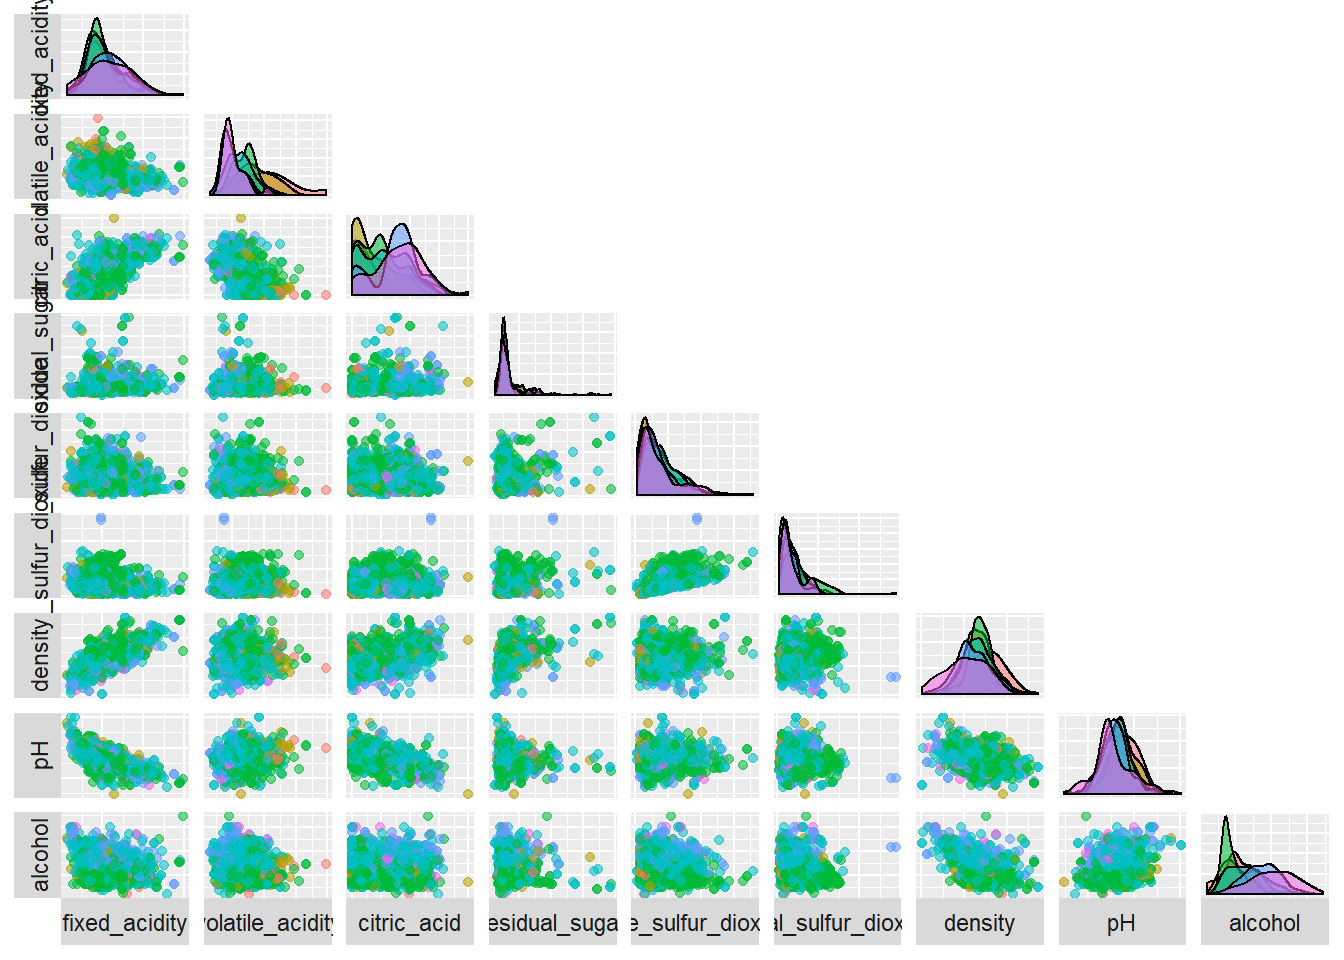
\includegraphics{class2_files/figure-beamer/unnamed-chunk-5-1.pdf}

\end{block}

\end{frame}

\begin{frame}[fragile]

\begin{block}{Componentes Principales 7:}

\begin{Shaded}
\begin{Highlighting}[]
\CommentTok{# summary method}
\KeywordTok{summary}\NormalTok{(ir.pca)}
\end{Highlighting}
\end{Shaded}

\begin{verbatim}
## Importance of components:
##                           PC1    PC2     PC3     PC4
## Standard deviation     1.7125 0.9524 0.36470 0.16568
## Proportion of Variance 0.7331 0.2268 0.03325 0.00686
## Cumulative Proportion  0.7331 0.9599 0.99314 1.00000
\end{verbatim}

El metodo summary describe la importancia de las componentes
principales. La primera columna describe la importancia de las PCs, la
segundo la fracccion de la varianza en los datos, explicada por cada
componente y la tercera porcion cumulativa de la varianza de los datos.

\end{block}

\end{frame}

\begin{frame}[fragile]

\begin{block}{Componentes Principales 8:}

\begin{Shaded}
\begin{Highlighting}[]
\KeywordTok{plot}\NormalTok{(ir.pca}\OperatorTok{$}\NormalTok{x[,}\DecValTok{1}\OperatorTok{:}\DecValTok{2}\NormalTok{], }\DataTypeTok{col=}\NormalTok{ ir.species)}
\end{Highlighting}
\end{Shaded}

\includegraphics{class2_files/figure-beamer/unnamed-chunk-7-1.pdf}

\end{block}

\end{frame}

\begin{frame}

\begin{block}{Seleccion de Features}

\end{block}

\begin{block}{Un poco de clasificacion usando los vecinos:}

\begin{itemize}
\item
  Se uttiliza para clasificar nuevos ejemplo asignandoles la clase de
  los ejemplos mas similares.
\item
  Se utiliza exitosamente en reconocimiento de caracteresen imagenes y
  video (CV), ver por ejemplo \textless{}www.opencv.org\textgreater{}
\item
  predecir si una dada persona le gustara cierta pelicula como por ej en
  el Netflix challenge
  \url{https://www.kaggle.com/netflix-inc/netflix-prize-data}.
\item
  Identificar patrones en datos geneticos, para detectar proteinas
  especificas o enfermedades.
\end{itemize}

En general los NN (Nearest Neighbours) clasificadores son muy adecuados
cuando las relaciones entre features y clases objetivo son complicadas,
numerosas o dificiles de entender.

\end{block}

\end{frame}

\begin{frame}

\begin{block}{The kNN algorithm:}

\begin{itemize}
\item
  Fortalezas: Simple y efectivo, rapido de entrenar
\item
  Debilidades: no da un modelo, lento para clasificar, costoso en
  memoria.
\item
  Para cada dato en el conjunto a clasificar, kNN identifica k datos en
  el conjunto de datos ya clasificado (de entrenamiento) que estan
  ``cerca'', donde k es un numero especificado.
\item
  Para localizar un punto como vecino se requiere una funcion distancia,
  como la distancia Euclidiana o la distancia Manhattan, leer sobre esto
  usando ?dist.
\item
  El dato a clasificar es asignado a la clase de la mayoria de sus
  k-vecinos.
\end{itemize}

\end{block}

\end{frame}

\begin{frame}

\begin{block}{Eligiendo el numero apropiado de vecinos:}

\begin{itemize}
\tightlist
\item
  Esta relacionado con un problema muy importante. Elegir un k grande
  puede reducir el impacto causado por datos muy ruidosos, pero asi
  tambien se corre el riesgo de ignorar patrones locales importante
  (superficie o borde de decision).
\end{itemize}

\begin{figure}
\centering
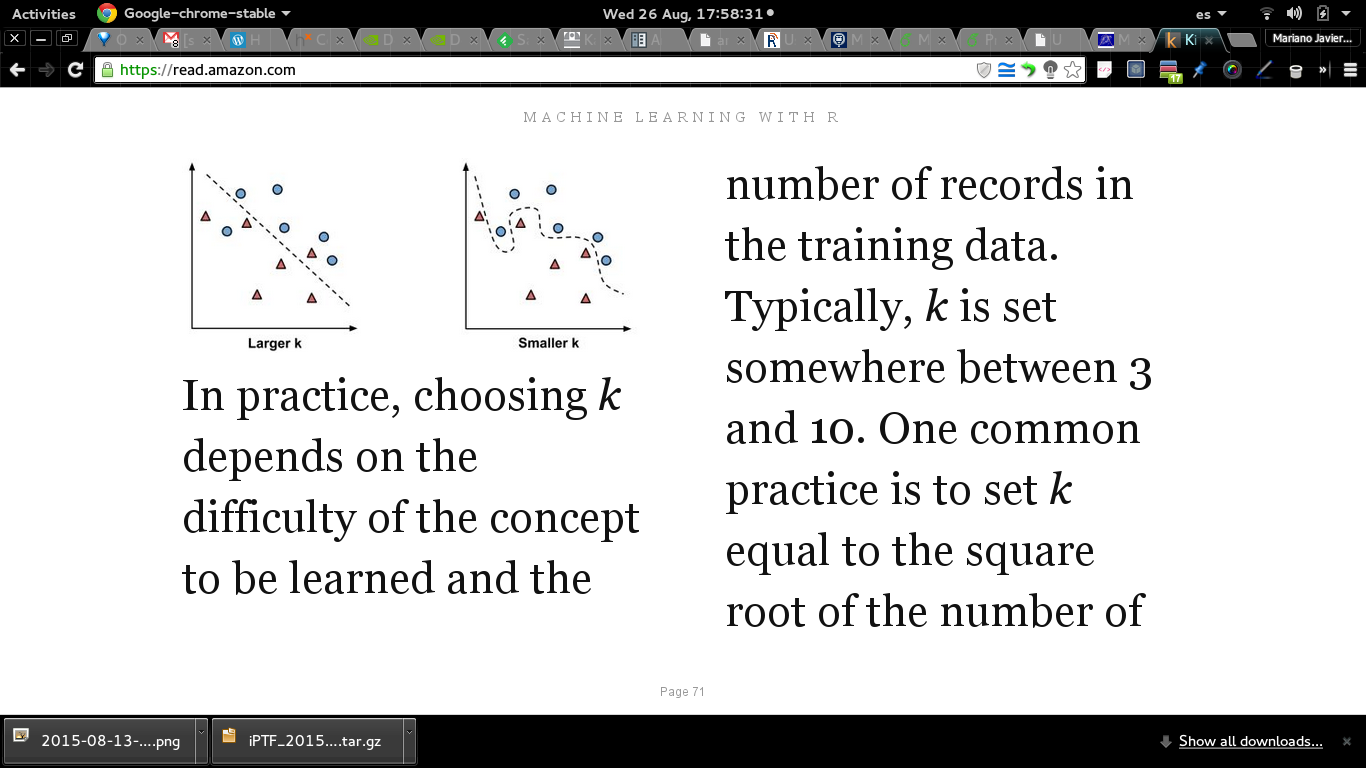
\includegraphics{./number-of-knn.png}
\caption{}
\end{figure}

\end{block}

\end{frame}

\begin{frame}

\begin{block}{Preparando los datos para un algoritmo:}

\begin{itemize}
\item
  Los Features son tipicamente transformados a una medida estandar
  previamente a la aplicacion de un algoritmo como kNN. La razon de esto
  es que la formula de distancia es afectada por como son medidos los
  features.
\item
  En particular si ciertos features tienen valores mucho mayores que
  otros, las mediciones de distancia seran muy fuertemente dominadas por
  los valores mas grandes.
\item
  Lo que se necesita es una manera de lograr que todos los features
  contribuyan equitativamente a la formula de distancia.
\end{itemize}

\end{block}

\end{frame}

\begin{frame}

\begin{block}{Rescalando los features}

El metodo tradicional para kNN es la \textbf{minimizacion minmax}. Este
proceso transforma cada feature de forma tal que todos sus valores
caigan entre 0 y 1.

Otra transformacion comun es llamada la \textbf{z-score normalization}.
Que consiste en substraer a cada dato la media del mismo y dividirla por
su desviacion estandart, quedando entonces en algun rango de numeros
negativos a positivos.

La formula de la distancia Euclidea no esta definida para datos
nominales, por lo que es necesario convertir cada feature nominal en
algun formato numerico. Como por ejemplo con \textbf{dummy coding}.

\end{block}

\end{frame}

\begin{frame}[fragile]

\begin{block}{Diagnosticando Cancer:}

\begin{itemize}
\tightlist
\item
  Investigaremos ahora la utilidad del ML para detectar cancer aplicando
  el algoritmo kNN a mediciones de biopsias de mujeres, utilizando el
  conjunto de datos ``Breast Cancer Winscosin Diagnostic'' del UCI ML
  Repository \url{http://archive.ics.uci.edu/ml} que incluye 569
  ejemplos de biopsias, en cada una se midieron 32 features (diferentes
  caracteristicas de las nucleos celulares) y el diagnostico codificado
  como M (Maligno) o B (Benigno).
\end{itemize}

\begin{Shaded}
\begin{Highlighting}[]
\NormalTok{data <-}\StringTok{ }\KeywordTok{read.csv}\NormalTok{(}\StringTok{"http://archive.ics.uci.edu/ml/machine-learning-databases/breast-cancer-wisconsin/wdbc.data"}\NormalTok{,}\DataTypeTok{header=}\OtherTok{FALSE}\NormalTok{)}
\NormalTok{data <-}\StringTok{ }\NormalTok{data[}\OperatorTok{-}\DecValTok{1}\NormalTok{]}
\KeywordTok{str}\NormalTok{(data)}
\end{Highlighting}
\end{Shaded}

\begin{verbatim}
## 'data.frame':    569 obs. of  31 variables:
##  $ V2 : Factor w/ 2 levels "B","M": 2 2 2 2 2 2 2 2 2 2 ...
##  $ V3 : num  18 20.6 19.7 11.4 20.3 ...
##  $ V4 : num  10.4 17.8 21.2 20.4 14.3 ...
##  $ V5 : num  122.8 132.9 130 77.6 135.1 ...
##  $ V6 : num  1001 1326 1203 386 1297 ...
##  $ V7 : num  0.1184 0.0847 0.1096 0.1425 0.1003 ...
##  $ V8 : num  0.2776 0.0786 0.1599 0.2839 0.1328 ...
##  $ V9 : num  0.3001 0.0869 0.1974 0.2414 0.198 ...
##  $ V10: num  0.1471 0.0702 0.1279 0.1052 0.1043 ...
##  $ V11: num  0.242 0.181 0.207 0.26 0.181 ...
##  $ V12: num  0.0787 0.0567 0.06 0.0974 0.0588 ...
##  $ V13: num  1.095 0.543 0.746 0.496 0.757 ...
##  $ V14: num  0.905 0.734 0.787 1.156 0.781 ...
##  $ V15: num  8.59 3.4 4.58 3.44 5.44 ...
##  $ V16: num  153.4 74.1 94 27.2 94.4 ...
##  $ V17: num  0.0064 0.00522 0.00615 0.00911 0.01149 ...
##  $ V18: num  0.049 0.0131 0.0401 0.0746 0.0246 ...
##  $ V19: num  0.0537 0.0186 0.0383 0.0566 0.0569 ...
##  $ V20: num  0.0159 0.0134 0.0206 0.0187 0.0188 ...
##  $ V21: num  0.03 0.0139 0.0225 0.0596 0.0176 ...
##  $ V22: num  0.00619 0.00353 0.00457 0.00921 0.00511 ...
##  $ V23: num  25.4 25 23.6 14.9 22.5 ...
##  $ V24: num  17.3 23.4 25.5 26.5 16.7 ...
##  $ V25: num  184.6 158.8 152.5 98.9 152.2 ...
##  $ V26: num  2019 1956 1709 568 1575 ...
##  $ V27: num  0.162 0.124 0.144 0.21 0.137 ...
##  $ V28: num  0.666 0.187 0.424 0.866 0.205 ...
##  $ V29: num  0.712 0.242 0.45 0.687 0.4 ...
##  $ V30: num  0.265 0.186 0.243 0.258 0.163 ...
##  $ V31: num  0.46 0.275 0.361 0.664 0.236 ...
##  $ V32: num  0.1189 0.089 0.0876 0.173 0.0768 ...
\end{verbatim}

\end{block}

\end{frame}

\begin{frame}[fragile]

\begin{block}{Entendiendo los datos:}

Independientemente del metodo de ML aplicado, las variables de
identificacion \textbf{deben} ser excluidas. No hacerlo puede llevar a
hallazgos erroneos a causa de que la identificacion puede ser utilizada
para predecir muy bien. La siguiente variable, el diagnostico es de
particular interes, por que es lo que se quiere predecir.

\begin{Shaded}
\begin{Highlighting}[]
\KeywordTok{table}\NormalTok{(data}\OperatorTok{$}\NormalTok{V2)}
\end{Highlighting}
\end{Shaded}

\begin{verbatim}
## 
##   B   M 
## 357 212
\end{verbatim}

Ya que estamos miremos el resto de las variables, sus rangos etc.

\begin{Shaded}
\begin{Highlighting}[]
\KeywordTok{summary}\NormalTok{(data)}
\end{Highlighting}
\end{Shaded}

\begin{verbatim}
##  V2            V3               V4              V5        
##  B:357   Min.   : 6.981   Min.   : 9.71   Min.   : 43.79  
##  M:212   1st Qu.:11.700   1st Qu.:16.17   1st Qu.: 75.17  
##          Median :13.370   Median :18.84   Median : 86.24  
##          Mean   :14.127   Mean   :19.29   Mean   : 91.97  
##          3rd Qu.:15.780   3rd Qu.:21.80   3rd Qu.:104.10  
##          Max.   :28.110   Max.   :39.28   Max.   :188.50  
##        V6               V7                V8                V9         
##  Min.   : 143.5   Min.   :0.05263   Min.   :0.01938   Min.   :0.00000  
##  1st Qu.: 420.3   1st Qu.:0.08637   1st Qu.:0.06492   1st Qu.:0.02956  
##  Median : 551.1   Median :0.09587   Median :0.09263   Median :0.06154  
##  Mean   : 654.9   Mean   :0.09636   Mean   :0.10434   Mean   :0.08880  
##  3rd Qu.: 782.7   3rd Qu.:0.10530   3rd Qu.:0.13040   3rd Qu.:0.13070  
##  Max.   :2501.0   Max.   :0.16340   Max.   :0.34540   Max.   :0.42680  
##       V10               V11              V12               V13        
##  Min.   :0.00000   Min.   :0.1060   Min.   :0.04996   Min.   :0.1115  
##  1st Qu.:0.02031   1st Qu.:0.1619   1st Qu.:0.05770   1st Qu.:0.2324  
##  Median :0.03350   Median :0.1792   Median :0.06154   Median :0.3242  
##  Mean   :0.04892   Mean   :0.1812   Mean   :0.06280   Mean   :0.4052  
##  3rd Qu.:0.07400   3rd Qu.:0.1957   3rd Qu.:0.06612   3rd Qu.:0.4789  
##  Max.   :0.20120   Max.   :0.3040   Max.   :0.09744   Max.   :2.8730  
##       V14              V15              V16               V17          
##  Min.   :0.3602   Min.   : 0.757   Min.   :  6.802   Min.   :0.001713  
##  1st Qu.:0.8339   1st Qu.: 1.606   1st Qu.: 17.850   1st Qu.:0.005169  
##  Median :1.1080   Median : 2.287   Median : 24.530   Median :0.006380  
##  Mean   :1.2169   Mean   : 2.866   Mean   : 40.337   Mean   :0.007041  
##  3rd Qu.:1.4740   3rd Qu.: 3.357   3rd Qu.: 45.190   3rd Qu.:0.008146  
##  Max.   :4.8850   Max.   :21.980   Max.   :542.200   Max.   :0.031130  
##       V18                V19               V20          
##  Min.   :0.002252   Min.   :0.00000   Min.   :0.000000  
##  1st Qu.:0.013080   1st Qu.:0.01509   1st Qu.:0.007638  
##  Median :0.020450   Median :0.02589   Median :0.010930  
##  Mean   :0.025478   Mean   :0.03189   Mean   :0.011796  
##  3rd Qu.:0.032450   3rd Qu.:0.04205   3rd Qu.:0.014710  
##  Max.   :0.135400   Max.   :0.39600   Max.   :0.052790  
##       V21                V22                 V23             V24       
##  Min.   :0.007882   Min.   :0.0008948   Min.   : 7.93   Min.   :12.02  
##  1st Qu.:0.015160   1st Qu.:0.0022480   1st Qu.:13.01   1st Qu.:21.08  
##  Median :0.018730   Median :0.0031870   Median :14.97   Median :25.41  
##  Mean   :0.020542   Mean   :0.0037949   Mean   :16.27   Mean   :25.68  
##  3rd Qu.:0.023480   3rd Qu.:0.0045580   3rd Qu.:18.79   3rd Qu.:29.72  
##  Max.   :0.078950   Max.   :0.0298400   Max.   :36.04   Max.   :49.54  
##       V25              V26              V27               V28         
##  Min.   : 50.41   Min.   : 185.2   Min.   :0.07117   Min.   :0.02729  
##  1st Qu.: 84.11   1st Qu.: 515.3   1st Qu.:0.11660   1st Qu.:0.14720  
##  Median : 97.66   Median : 686.5   Median :0.13130   Median :0.21190  
##  Mean   :107.26   Mean   : 880.6   Mean   :0.13237   Mean   :0.25427  
##  3rd Qu.:125.40   3rd Qu.:1084.0   3rd Qu.:0.14600   3rd Qu.:0.33910  
##  Max.   :251.20   Max.   :4254.0   Max.   :0.22260   Max.   :1.05800  
##       V29              V30               V31              V32         
##  Min.   :0.0000   Min.   :0.00000   Min.   :0.1565   Min.   :0.05504  
##  1st Qu.:0.1145   1st Qu.:0.06493   1st Qu.:0.2504   1st Qu.:0.07146  
##  Median :0.2267   Median :0.09993   Median :0.2822   Median :0.08004  
##  Mean   :0.2722   Mean   :0.11461   Mean   :0.2901   Mean   :0.08395  
##  3rd Qu.:0.3829   3rd Qu.:0.16140   3rd Qu.:0.3179   3rd Qu.:0.09208  
##  Max.   :1.2520   Max.   :0.29100   Max.   :0.6638   Max.   :0.20750
\end{verbatim}

\end{block}

\end{frame}

\begin{frame}[fragile]

\begin{block}{Transformacion de los datos:}

Necesitamos crear una funcion normalizacion en R:

\begin{Shaded}
\begin{Highlighting}[]
\NormalTok{normalize <-}\StringTok{ }\ControlFlowTok{function}\NormalTok{(x) \{}
  \KeywordTok{return}\NormalTok{ ((x}\OperatorTok{-}\KeywordTok{min}\NormalTok{(x))}\OperatorTok{/}\NormalTok{(}\KeywordTok{max}\NormalTok{(x)}\OperatorTok{-}\KeywordTok{min}\NormalTok{(x)))}
\NormalTok{\}}
\end{Highlighting}
\end{Shaded}

Despues de ejecutar el codigo previo, la funcion esta disponible para
sus uso. Veamos si funciona en algunos vectores.

\begin{Shaded}
\begin{Highlighting}[]
\KeywordTok{normalize}\NormalTok{(}\KeywordTok{c}\NormalTok{(}\DecValTok{1}\NormalTok{,}\DecValTok{2}\NormalTok{,}\DecValTok{3}\NormalTok{,}\DecValTok{4}\NormalTok{,}\DecValTok{5}\NormalTok{))}
\end{Highlighting}
\end{Shaded}

\begin{verbatim}
## [1] 0.00 0.25 0.50 0.75 1.00
\end{verbatim}

\begin{Shaded}
\begin{Highlighting}[]
\KeywordTok{normalize}\NormalTok{(}\KeywordTok{c}\NormalTok{(}\DecValTok{10}\NormalTok{,}\DecValTok{20}\NormalTok{,}\DecValTok{30}\NormalTok{,}\DecValTok{40}\NormalTok{,}\DecValTok{50}\NormalTok{))}
\end{Highlighting}
\end{Shaded}

\begin{verbatim}
## [1] 0.00 0.25 0.50 0.75 1.00
\end{verbatim}

No podemos aplicar la funcion a los features numericos del dataframe
directamente.

\end{block}

\end{frame}

\begin{frame}[fragile]

\begin{block}{Transformacion de los datos:}

La funcion lapply() de R toma una lista y aplica una funcion a cada
elemento de la lista.

\begin{Shaded}
\begin{Highlighting}[]
\NormalTok{data_n <-}\StringTok{ }\KeywordTok{as.data.frame}\NormalTok{(}\KeywordTok{lapply}\NormalTok{(data[}\DecValTok{2}\OperatorTok{:}\DecValTok{31}\NormalTok{], normalize))}
\KeywordTok{summary}\NormalTok{(data_n}\OperatorTok{$}\NormalTok{V3)}
\end{Highlighting}
\end{Shaded}

\begin{verbatim}
##    Min. 1st Qu.  Median    Mean 3rd Qu.    Max. 
##  0.0000  0.2233  0.3024  0.3382  0.4164  1.0000
\end{verbatim}

\begin{Shaded}
\begin{Highlighting}[]
\KeywordTok{summary}\NormalTok{(data_n}\OperatorTok{$}\NormalTok{V8)}
\end{Highlighting}
\end{Shaded}

\begin{verbatim}
##    Min. 1st Qu.  Median    Mean 3rd Qu.    Max. 
##  0.0000  0.1397  0.2247  0.2606  0.3405  1.0000
\end{verbatim}

Bingo! En ausencia de nuevos datos de laboratorio, vamos a simular este
escenario dividiendo nuestros datos en una \textbf{muestra de
entrenamiento} que usaremos para construir el modelo kNN y una
\textbf{muestra de validacion} que usaremos para medir la presicion
predictiva del mismo.

\end{block}

\end{frame}

\begin{frame}[fragile]

\begin{block}{Entrenando un clasificador:}

Notese que dichos conjuntos de datos deben ser representativos del
conjunto de datos, i.e. \textbf{metodos de muestreo aleatorios}!

\begin{Shaded}
\begin{Highlighting}[]
\NormalTok{data_train <-}\StringTok{ }\NormalTok{data_n[}\DecValTok{1}\OperatorTok{:}\DecValTok{469}\NormalTok{, ]}
\NormalTok{data_test  <-}\StringTok{ }\NormalTok{data_n[}\DecValTok{470}\OperatorTok{:}\DecValTok{569}\NormalTok{, ] }
\end{Highlighting}
\end{Shaded}

Excluimos la variable objetivo (Benigno/Maligno), pero necesitamos
guardar estos factores en vectores!

\begin{Shaded}
\begin{Highlighting}[]
\NormalTok{data_train_labels <-}\StringTok{ }\NormalTok{data[}\DecValTok{1}\OperatorTok{:}\DecValTok{469}\NormalTok{, }\DecValTok{1}\NormalTok{]}
\NormalTok{data_test_labels  <-}\StringTok{ }\NormalTok{data[}\DecValTok{470}\OperatorTok{:}\DecValTok{569}\NormalTok{, }\DecValTok{1}\NormalTok{]}
\end{Highlighting}
\end{Shaded}

Para el algoritmo kNN la fase de entrenamiento no involucra construir un
modelo, para clasificar nuestros datos de validacion utilizaremos el
paquete class, instalarlo ia!

La datps de validacion son clasificados tomando los votos entre los k
vecinos mas cercanos del conjunto de entrenamiento. Si hay empate se
decide aleatoriamente. Entonces usamos la funcion knn() para clasificar.

\end{block}

\end{frame}

\begin{frame}[fragile]

\begin{block}{Evaluando la performance del modelo.}

\begin{Shaded}
\begin{Highlighting}[]
\KeywordTok{library}\NormalTok{(class)}
\NormalTok{data_test_pred <-}\StringTok{ }\KeywordTok{knn}\NormalTok{(}\DataTypeTok{train=}\NormalTok{data_train, }\DataTypeTok{test=}\NormalTok{data_test, }\DataTypeTok{cl=}\NormalTok{data_train_labels, }\DataTypeTok{k=}\DecValTok{21}\NormalTok{)}
\end{Highlighting}
\end{Shaded}

El siguiente paso en el proceso es evaluar como las clases predichas en
data\_test\_pred se condicen con los valores verdaderos en el vector
data\_test\_labels.

\begin{Shaded}
\begin{Highlighting}[]
\KeywordTok{library}\NormalTok{(gmodels)}
\KeywordTok{CrossTable}\NormalTok{(}\DataTypeTok{x=}\NormalTok{data_test_labels, }\DataTypeTok{y=}\NormalTok{data_test_pred, }\DataTypeTok{prop.chisq =} \OtherTok{FALSE}\NormalTok{)}
\end{Highlighting}
\end{Shaded}

\begin{verbatim}
## 
##  
##    Cell Contents
## |-------------------------|
## |                       N |
## |           N / Row Total |
## |           N / Col Total |
## |         N / Table Total |
## |-------------------------|
## 
##  
## Total Observations in Table:  100 
## 
##  
##                  | data_test_pred 
## data_test_labels |         B |         M | Row Total | 
## -----------------|-----------|-----------|-----------|
##                B |        77 |         0 |        77 | 
##                  |     1.000 |     0.000 |     0.770 | 
##                  |     0.975 |     0.000 |           | 
##                  |     0.770 |     0.000 |           | 
## -----------------|-----------|-----------|-----------|
##                M |         2 |        21 |        23 | 
##                  |     0.087 |     0.913 |     0.230 | 
##                  |     0.025 |     1.000 |           | 
##                  |     0.020 |     0.210 |           | 
## -----------------|-----------|-----------|-----------|
##     Column Total |        79 |        21 |       100 | 
##                  |     0.790 |     0.210 |           | 
## -----------------|-----------|-----------|-----------|
## 
## 
\end{verbatim}

\end{block}

\end{frame}

\begin{frame}

\begin{block}{Ejercicios.}

Los valores correctos estan en la diagonal de la matriz, 98\% de
precision para unas pocas lineas de R!

\begin{itemize}
\item
  Mejore el rendimiento utilizando una normalizacion con z-scores
  provista por la funcion scale() de R.
\item
  Pruebe algunos valores alternativos de k=1, 5, 11, 15, 21 y seleccione
  el mejor valor de k.
\item
  mientras termina su merecido cafe verifique si el resultado cambia
  utilizando paciente elegidos aleatoriamente para el conjunto de
  validacion.
\end{itemize}

\end{block}

\end{frame}

\begin{frame}

\end{frame}

\begin{frame}

\begin{block}{Una breve excursion en dimensiones mas altas:}

\textbf{Ajustar} una funcion (como el modelo lineal) nos permite
generalizar nuestra estima de la funcion densidad mas alla de los puntos
medidos, pero no nos permite manejar otras generalizaciones bien.

Un primer problema es que tipo de funciones necesitamos para
representar, consideren por ejemplo unos puntos distribuidos en una
superficie de baja dimensionalidad en un espacio de dimensionalidad
mayor, por ejemplo una hoja de cuaderno en 3D. En la direccion
perpendicular a la superficie la distribucion es muy angosta, algo que
es dificil de expandir con funciones bases trigonometricas o
polinomicas.

Este problema es muy comun, en un espacio de features de alta
dimensionalidad toda distribucion se vuelve superficial. Para entender
este concepto, considere el volumen de una hiper esfera de radio \(r\)
en un espacio de dimension \(d\):

\[V(r)=\frac{\pi^{d/2}r^{d}}{(d/2)!}\]

los factoriales no enteros estan definidos por la funcion
\[\Gamma(n+1)=n!\].

\end{block}

\end{frame}

\begin{frame}

\begin{block}{y los problemas de las distribuciones alli.}

Ahora miremos a la fraccion de volumen que ocupa una cascara de ancho
\(\epsilon\), comparada al volumen total de la esfera, en el limite
cuando \[d \rightarrow \infty\]: \[
\frac{V(r)-V(r-\epsilon)}{V(r)}=\frac{r^{d}-(r-\epsilon)^{d}}{r^{d}}=1-(1-\frac{r}{d})=1
\] Cuando d crece, todo el volumen esta en una cascara fina sobre la
superficie.

Ahora considere lo que implica esto para una una coleccion de puntos que
provienen de una distribucion: puntos tipicos provienen de una
distribucion no de los bordes, pero en un espacio de alta
dimensionalidad las distribuciones son esencialmente bordes y los
analisis estaran dominados por los efectos de borde.

Otro punto importante es puede que no podamos muestrear bien la
distribucion alli.

\end{block}

\end{frame}

\begin{frame}

\begin{block}{Using mixture models for clustering}

Dados los problemas de estimacion mencionados, una posible solucion es
proponer por ejemplo poner alguna distribucion (Gaussiana por ejemplo)
en cada punto medido, esto se conoce como \textbf{Kernel density
estimation}.

Una mejor aproximacion seria encontrar lugares interesantes donde poner
un numero chico (respecto al numero de datos) donde poner algunas
funciones locales que modelen bien su vecindad. Esto se conoce como
\textbf{mixture models}.

Esto esta conectado con el problema de partir un conjunto de datos
aglomerando o \textbf{clustering}, que es un ejemplo de
\textbf{aprendizaje no supervisado}. A diferencia de los metodos de
fiteo con una funcion distribucion determinada, el algoritmo debe
aprender por si mismo donde estan esos lugares interesantes en el
conjunto de datos.

Importantes aplicaciones de estos algoritmos se encuentran en la
compresion de datos, la deteccion de outliers y crear clasificadores
generativos, donde se modela cada densidad de clase \(p(x|y = c)\) por
una mixtura.

\end{block}

\end{frame}

\begin{frame}

\begin{block}{Mixturas de Gausianas en D dimensiones:}

un modelo de mixturas puede escribirse factorizando la densidad sobre
multiples Gaussianas:

\[p(\bar{x})=\sum_{m=1}^{M}p(\bar{x}, c_{m})=\sum_{m=1}^{M}p(\bar{x}|c_{m})p(c_{m})\]

\[p(\bar{x})=\sum_{m=1}^{M} \frac{|C_{m}^{-1}|^{1/2}}{(2 \pi)^{D/2}} \exp[{-(\bar{x}-\bar{\mu})^{T}.C_{M}^{-1}.(\bar{x}-(\bar{\mu}))/2}]p(c_{m})\]

donde \(|.|^{1/2}\) es la raiz cuadrada del determinante, y \(c_{m}\) se
refieren a la \(m\)-esima Gaussiana con media \(\mu_{m}\) y matriz de
covarianza \(C_{m}\). El desafio es por supuesto encontrar esos
parametros!

\end{block}

\end{frame}

\begin{frame}

\begin{block}{Mixturas de Gausianas en D dimensiones:}

Si tenemos una sola Gaussiana, el valor medio \(\mu\) puede ser estimado
simplemente promediando los los datos:
\[ \bar{\mu}=\int_{-\infty}^{\infty} \bar{x} p(\bar{x}) d\bar{x} \simeq \frac{1}{N} \sum_{n=1}^{N} \bar{x}_{n}\]

dado que una integral sobre una funcion densidad de probabilidad puede
aproximarse por una suma de variables extraidas de la distribucion
(importante recordar). Todavia no la conocemos a la funcion
distribucion, pero por definicion es de donde nuestro conjunto de datos
fue extraido.

La idea puede extenderse a mas Gaussianas reconociendo que la \(m\)esima
media es la integral respecto a la distribucion condicional:
\[\bar{\mu}=\int \bar{x} p(\bar{x} | c_{m}) d\bar{x} = \int \bar{x} \frac{p(c_{m}|\bar{x})}{p(c_m)}p(\bar{x})d(\bar{x}) \simeq \frac{1}{Np(c_{m})}\sum_{n=1}^{N} \bar{x}_{n} p(c_{m} | \bar{x}_{n})\]

\end{block}

\end{frame}

\begin{frame}

\begin{block}{Mixturas de Gausianas en D dimensiones:}

de forma similar se puede encontrar que la matriz de covarianza es:

\[ C_{m} \simeq \frac{1}{N p(c_{m})} \sum_{n+1}^{N} (\bar{x}_{n}-\bar{\mu}_{m})(\bar{x}_{n}-\bar{\mu}_{m})^{T} p(c_{m}| x_{n})\]

y los pesos en la expansion por,

\[ p(c_{m})=\int_{-\infty}^{\infty} p(\bar{x}, c_{m}) d\bar{x}= \int_{-\infty}^{\infty} p(c_{m} | \bar{x}) p(\bar{x}) d{\bar{x}} \simeq \frac{1}{N} \sum_{i=1}^{N} p(c_{m} | \bar{x}_{n})\]
Pero, como encontramos la probabilidad posterior \(p(c_{m}|\bar{x})\)
utilizada en estas sumas? Por definicion es:

\end{block}

\end{frame}

\begin{frame}

\begin{block}{El Algoritmo EM}

\[ p(c_{m}| \bar{x})=\frac{p(\bar{x}, c_{m})}{p(\bar{x})}=\frac{p(\bar{x}| c_{m})p(c_{m})}{\sum_{m=1}^{M} p(\bar{x}|c_{m})p(c_{m})}
\]

lo cual puede calcularse segun el modelo inicial propuesto. Esto puede
sonar a un razonamiento circular y lo es! Las probabilidades de los
puntos pueden ser calculados si conocemos los parametros de las
distribuciones (medias, varianzas, pesos) y los parametros pueden ser
encontrados si conocemos las probabilidades.

Como comenzamos no conociendo nada, comenzamos suponiendo los parametros
aleatoriamente y vamos y venimos iterativamente computando
iterativamente las probabilidades y los parametros.

\end{block}

\end{frame}

\begin{frame}

\begin{block}{El algoritmo EM y sus parientes:}

Calculando una distribucion esperada dados los parametros y luego
encontrando los parametros mas probables dada una distribucion, es
llamado el algoritmo de maximizacion de expectacion EM y este converge a
una distribucion de maximo likelihood comenzando con una semilla
aleatoria.

Las Gaussianas pueden por ejemplo ser inicializadas con medias
aleatorias y varianzas lo suficientemente grandes como para ``sentir''
el conjunto de datos. El problema es que las Gausianas captura solo
proximidad, el problema surge cuando hay superposicion de las mismas o
alguna colapsa.

Una mejor alternativa es basar la expansion de la funcion distribucion
alrededor de modelos que pueden capturar mejor la complejidad
localmente. Esta poderosa idea ha llevado ha desarrollar diferentes
algoritmos como: \textbf{redes Bayesianas}, \textbf{mixtures of experts}
o \textbf{cluster wigthed models}.

\end{block}

\end{frame}

\begin{frame}

\begin{block}{El algoritmo EM, una aplicacion:}

\includegraphics{class2_files/figure-beamer/unnamed-chunk-18-1.pdf}

\end{block}

\end{frame}

\begin{frame}[fragile]

\begin{block}{El algoritmo EM, una aplicacion:}

\begin{verbatim}
## Package 'mclust' version 5.4
## Type 'citation("mclust")' for citing this R package in publications.
\end{verbatim}

Ahora se utilizan las ecuaciones definidas anteriormente para calcular

\begin{Shaded}
\begin{Highlighting}[]
\CommentTok{# Select 4 continuous variables and look for three distinct groups.}
\NormalTok{mcl.model <-}\StringTok{ }\KeywordTok{Mclust}\NormalTok{(iris[, }\DecValTok{1}\OperatorTok{:}\DecValTok{4}\NormalTok{], }\DecValTok{3}\NormalTok{)}
\CommentTok{# Plot our results.}
\KeywordTok{plot}\NormalTok{(mcl.model, }\DataTypeTok{what =} \StringTok{"classification"}\NormalTok{, }\DataTypeTok{main =} \StringTok{"Mclust Classification"}\NormalTok{)}
\end{Highlighting}
\end{Shaded}

\includegraphics{class2_files/figure-beamer/unnamed-chunk-20-1.pdf}

\end{block}

\end{frame}

\begin{frame}

\begin{block}{Mixturas de expertos:}

Tambien podemos usar modelos de mixturas para crear modelos
discriminativos de clasificacion y regresion. Por ejemplo consideren los
siguientes datos, parece una buena idea usar tres modelos diferentes de
regresion lineal, cada una aplicada a diferentes partes del espacio de
inputs. Esto puede modelarse si permitimos que los pesos de la mixtura y
las densidades sean dependientes del input.

\begin{figure}
\centering
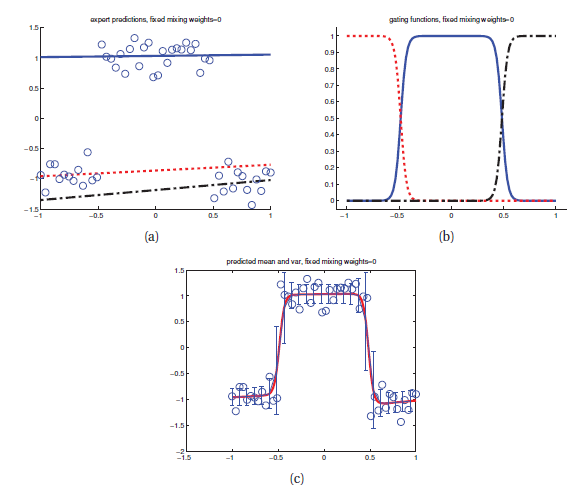
\includegraphics{./mix.png}
\caption{}
\end{figure}

\end{block}

\end{frame}

\begin{frame}

\begin{block}{un poco mas sobre Mixturas:}

La idea en una mixtura de expertos es que cada submodelo es considerado
un \textbf{experto} en cierta region del espacio de los inputs. La
funcion: \(p(z_{i} = k|x_{i}, \theta)\) is llamada funcion gatillo y
decide que experto usar en cada rango segun:
\(p(y_{i}|x_{i}, \theta)=\sum_{k} p(z_{i}=k|x_{i}, \theta) p(y_{i}|x_{i}, z_{i}=k, \theta)\).

Resulta claro que podemos ``pegar'' cualquier \textbf{arquitectura} como
un experto. Por ejemplo a veces se utilizan redes neuronales para
representar los expertos y las funciones gatillos, el resultado es
conocido como \textbf{mixture density network}. Son modelos lentos para
entrenar pero muy flexibles.

Las mixturas de expertos son muy utiles para resolver \textbf{problemas
de inversion} donde hay que invertir un mapeo de muchos a uno. Un
ejemplo tipico aparece en robotica, donde la localizacion de una mano
(robotica) \(y\) es unicamente determinada por los diferentes angulos
\(x\) de las articulaciones de un brazo robot. Sin embargo, para una
dada ubicacion y, hay muchas combinaciones de las articulaciones \(x\),
por lo que el mapeo inverso \(x = f^{-1}(y)\) no es unico. Otro ejemplo
seria en la identificacion posicional de gente en video, por los
problemas de auto ocultamiento etc.

\end{block}

\end{frame}

\begin{frame}

\begin{block}{Clustering hard K-means:}

Una variante particular del algoritmo EM para GMMs es conocido como el
\textbf{Algoritmo K-means}. Consideremos un modelo de mixturas
Gaussianas en el cual asumimos que:
\(\sum_{k} =\sigma^{2} \mathbb{I}_{D}\) y \(\pi_{k} = 1/K\) estan fijos,
por lo que solamente los centros de los cumulos,
\(\mu_{k} \in \mathbb{R}^{D}\), tienen que ser estimados.

Si consideramos la aproximacion de
\(p(z_{i}=k|x_{i}, \theta) \sim \mathbb{I}(k=z_{i}^{*})\),como
\(z_{i}^{*}= max_{k} p(z_{i}=k | x_{i}, \theta)\). obtenemos el llamado
\textbf{hard K-means}, donde estamos asignando cada punto de datos a un
cumulo. Dado que asumimos una matriz de covarianza esferica (en el
espacio de features) para cada cumulo, el cumulo mas probable para cada
dato for \(x_{i}\) puede ser computado encontrando el cumulo propuesto
mas cercano en cada paso.

En cada paso, debemos encontrar las distancias entre los \(N\) puntos de
datos y los \(K\) centros de los cumulos lo que lleva un tiempo de orden
\(NKD\).Sin embargo esto puede acelerarse. Dada las asignaciones duras,
en cada paso puedo recalcular el centro de los cumulos computando la
media de todos los puntos asignados al mismo:
\(\mu_{k}=\frac{1}{N} \sum_{i:z_{i}=k} x_{i}\).

\end{block}

\end{frame}

\begin{frame}[fragile]

\begin{block}{ejemplo de K-means:}

\begin{Shaded}
\begin{Highlighting}[]
\KeywordTok{set.seed}\NormalTok{(}\DecValTok{20}\NormalTok{)}
\NormalTok{irisCluster <-}\StringTok{ }\KeywordTok{kmeans}\NormalTok{(iris[, }\DecValTok{3}\OperatorTok{:}\DecValTok{4}\NormalTok{], }\DecValTok{3}\NormalTok{, }\DataTypeTok{nstart =} \DecValTok{20}\NormalTok{)}
\NormalTok{irisCluster}
\end{Highlighting}
\end{Shaded}

\begin{verbatim}
## K-means clustering with 3 clusters of sizes 50, 52, 48
## 
## Cluster means:
##   Petal.Length Petal.Width
## 1     1.462000    0.246000
## 2     4.269231    1.342308
## 3     5.595833    2.037500
## 
## Clustering vector:
##   [1] 1 1 1 1 1 1 1 1 1 1 1 1 1 1 1 1 1 1 1 1 1 1 1 1 1 1 1 1 1 1 1 1 1 1 1
##  [36] 1 1 1 1 1 1 1 1 1 1 1 1 1 1 1 2 2 2 2 2 2 2 2 2 2 2 2 2 2 2 2 2 2 2 2
##  [71] 2 2 2 2 2 2 2 3 2 2 2 2 2 3 2 2 2 2 2 2 2 2 2 2 2 2 2 2 2 2 3 3 3 3 3
## [106] 3 2 3 3 3 3 3 3 3 3 3 3 3 3 2 3 3 3 3 3 3 2 3 3 3 3 3 3 3 3 3 3 3 2 3
## [141] 3 3 3 3 3 3 3 3 3 3
## 
## Within cluster sum of squares by cluster:
## [1]  2.02200 13.05769 16.29167
##  (between_SS / total_SS =  94.3 %)
## 
## Available components:
## 
## [1] "cluster"      "centers"      "totss"        "withinss"    
## [5] "tot.withinss" "betweenss"    "size"         "iter"        
## [9] "ifault"
\end{verbatim}

\end{block}

\end{frame}

\begin{frame}[fragile]

\begin{block}{ejemplo de K-means:}

\begin{verbatim}
##    
##     setosa versicolor virginica
##   1     50          0         0
##   2      0         48         4
##   3      0          2        46
\end{verbatim}

\includegraphics{class2_files/figure-beamer/unnamed-chunk-23-1.pdf}

\end{block}

\end{frame}

\begin{frame}{Clustering soft K-means:}

Cuando computamos la \(p(z_{i} = k|x_{i}, \theta)\), la probabilidad
posterior que el punto \(i\) pertenezca al cumulo \(k\), esta cantidad
se puede pensar como la \textbf{responsabilidad} del cumulo \(k\) por el
punto \(i\) la cual puede calcularse siguiendo la regla de Bayes :
\(r_{ik}=p(z_{i}=k|x_{i}, \theta)=\frac{p(z_{i}=k|\theta )p(x_{i}|z_{i}=k, \theta)}{\sum_{j=1}^{K} p(z_{i}=j|\theta)p(x_{i}|z_{i}=j, \theta)}\)

Este procedimiento es llamado \textbf{soft clustering}, y permite una
mejor clasificacion automatica. Por ejemplo usando una version
binarizada del conjunto de carateres digitalizados MNIST, se puede hacer
un clustering con \(k=10\) y visualizar los centroides, tal como vemos
el metodo descubre correctamente algunas clases de digitos, pero otros
no (discutir).

\begin{figure}
\centering
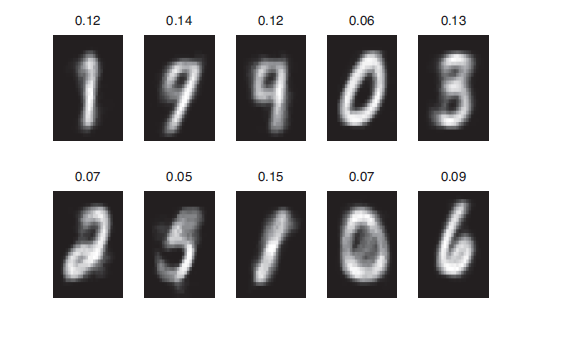
\includegraphics{./handw.png}
\caption{}
\end{figure}

\end{frame}

\begin{frame}

\begin{block}{Weapons of math destruction:}

Por mas detalles consultar el siguiente libro
\url{http://www.inference.org.uk/itprnn/book.html}.

Vale la pena mencionar tambien la posibilidad de llamar de python desde
R utilizando \url{https://rstudio.github.io/reticulate/} o trasnferir
dataframes a pandas y viceversa con
\url{https://github.com/wesm/feather} y el uso de ambos lenguajes en
sistemas distribuidos (Sparck).

Recuerde que los modelos por su naturaleza son simplificaciones, y
cuando lo creamos tomamos decisiones respecto que es importante incluir
(muchas veces en el proceso de seleccion de muestras) por lo que podemos
generar enormes puntos ciegos. Tenga en cuenta los posibles sesgos en
los conjuntos de datos, pq todo algoritmo los perpetuara y amplificara.

El reciente caso de Cambridge Analytics deberia llamar vuestra atencion
de los posibles mal usos de las tecnologias que desarrollamos, o los
problemas generados por el algoritmic trading, i.e the flash crack etc.

\end{block}

\end{frame}

\begin{frame}{La Ciencia de Datos es multidisciplinaria:}

\begin{figure}
\centering
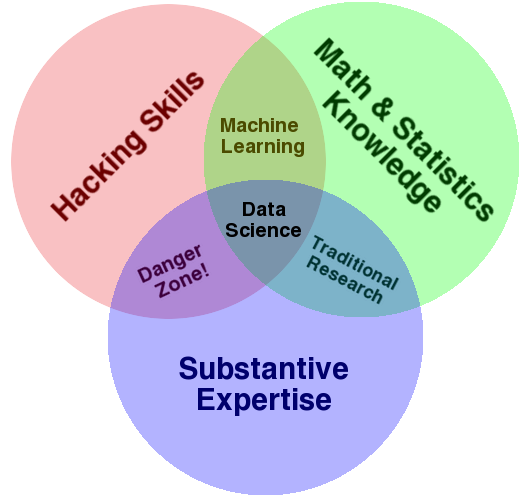
\includegraphics{./Data_Science_VD.png}
\caption{}
\end{figure}

\end{frame}

\begin{frame}{Practico 2: Entregar un Rmd donde se:}

\begin{itemize}
\item
  Elija un dataset clasificado de su preferencia y area (domain
  expertise), aplique un metodo de clustering y/o mixtura de Gaussianas
  en el mismo.
\item
  Investigue los resultados en el meta parametro \(K\) numero de cumulos
  e investigue posibles procesos de seleccion del mismo.
\item
  Elabore un resumen, y selecione un mejor valor segun el/los criterios
  aplicados, discuta el significado de los cumulos encontrados.
\item
  Comente la influencia de la normalizacion de los datos en los
  resultados del clustering.
\end{itemize}

\end{frame}

\end{document}
